\documentclass[./dissertation.tex]{subfiles}
\usepackage{multicol}

\begin{document}
    
    \contentchapter{Results}
    
    \section{General Experimental Configuration}
    Each set of experiments shares a similar hyperparameter search space. Below we describe the hyperparameters that are included in the search space of each experiment. 
    \subsection{Learning Rate (lr)}
    Through informal experimentation, we have found that the learning rate of 0.001 causes the models to converge consistently. The learning rate is thus set to 0.001 in each experiment.
    \subsection{Latent Space Dimensionality (lsdim)}
    Latent space dimensionality refers to the dimensionality of the vector output of the encoder of a DML network or the dimensionality of the posterior distribution of a VAE (also the dimensionality of the latent space). When the latent space dimensionality is 2, we see the added benefit of creating plots of the latent representations (though we can accomplish this through using dimensionality reduction methods like tSNE for higher dimensionalities as well). Example values for this hyperparameter used in experiments are 2, 4, and 10. 
    \subsection{Alpha}
    Alpha ($\alpha$) is a hyperapameter which refers to the balance between the unsupervised and supervised losses of some of the modified DML models. More details about the role of $\alpha$ in the model implementations are discussed in the methodology section of the model. Potential values for alpha are each between 0 (exclusive) and 1 (inclusive). We do not include 0 in this set as if $\alpha$ is set to 0, the model is equivalent to the fully supervised plain DML model because the supervised loss would not be included. If $\alpha$ is set to 1, then the model would train on only the unsupervised loss; for instance if the DML Autoencoder had $\alpha$ set to 1, then the model would be equivalent to an autoencoder. 
    \subsection{Partial Labels Percentage (pl\%)}
    The partial labels percentage hyperparameter refers to the percentage of the dataset that is labelled and thus the size of the partion of the dataset that can be used for labelled training. Of course, each of the datasets we use is fully labelled, so a partially labelled datset can be trivially constructed by ignoring some of the labels. As the sizes of the dataset vary, each percentage can refer to a different number of labelled samples. Values for the partial label percentage we use across experiments include 0.01, 0.1, 10, and 100 (with each value referring to the percentage). 
    \subsection{Datasets}
    Two datasets are used for evaluating the models. The first dataset is MNIST (\cite{lecun-mnisthandwrittendigit-2010}), a very popular dataset in machine learning containing greyscale images of handwritten digits. The second dataset we use is the organ OrganAMNIST dataset from MedMNIST v2 (\cite{medmnistv2}). This dataset contains 2D slices from computed tomography images from the Liver Tumor Segmentation Benchmark -- the labels correspond to the classification of 11 different body organs. The decision to use a second dataset was motivated because the as the claims are tested over more datasets, the results supporting the claims become more generalizable. The decision to use the OrganAMNIST dataset specifically is motivated in part due to the the Quinn Research Group working on similar tasks for biomedical imaging (\cite{Zain2020TowardsAU}). It is also motivated in part because OrganAMNIST is a more difficult dataset, at least for a the classfication task, as the leading accuracy for MNIST is .9991 (\cite{DBLP:journals/corr/abs-2008-10400}) while the leading accuracy for OrganAMNIST is .951 (\cite{medmnistv2}). The MNIST and OrganAMNIST datasets are similar in dimensionality (1 x 28 x 28), number of samples (60,000 and 58,850, respectively) and in that they are both greyscale.
    
    \begin{figure}[h]
        \centering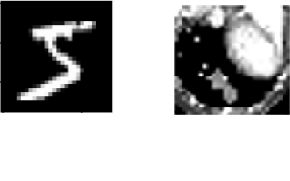
\includegraphics[width=0.5\textwidth]{figures/cropped_datasets.png}
        \caption{Sample images from the MNIST (left) and OrganAMNIST of MedMNIST (right) datasets}
        \label{Datasets Diagram}
    \end{figure}
    
    \subsection{Evaluation}
    We will evaluate the results by running each model on a test partition of data. We then take the latent points $Z$ generated by the model and the corresponding labels $Y$. Three classifiers (sklearn's implementation of RandomForest, MLP, and kNN) each output predicted labels $\hat{Y}$ for the latent points. In most of the charts shown, however, we only include the kNN classification output due to space constraints and the lack of meaningful difference between the output for each classifier. We finally measure the quality of the predicted labels $\hat{Y}$ using the Adjusted Mutual Information Score (AMI) (\cite{vinh2010information}) and accuracy (which is still helpful but is also easier to interpret in some cases). This scoring metric is common in research that looks to evaluate clustering performance (\cite{zhu2021finding})  (\cite{emmons2016analysis}). We will be using sklearn's implementation of AMI (\cite{scikit-learn}). The performance of a classifier on the latent points intuitively can be used as a measure of quality of clustering.
    \section{Claim 1: Benefits of Reconstruction Loss}
    In evaluating the first claim, we compare the performance of the plain DML model to the DML Autoencoder model. We do so by comparing the performance of the plain DML system and the DML Autoencoder across a search space containing the lsdim, alpha, and pl\% hyperparameters and both datasets.
   \begin{table}[]
       \centering
       \begin{tabular}{|c|c|c|c|}
            \hline
            \textbf{pl\%} & \textbf{lsdim} & \textbf{knn acc} & \textbf{knn MI}  \\
            \hline
            0.01 & 2 & 0.2603 & \textbf{0.1163} \\
            & & & \\ 
            & & & \\ 
            & & & \\ 
            & 10 & \textbf{0.2678} & 0.1126 \\ 
            & & & \\ 
            & & & \\ 
            & & & \\ 
            0.1 & 2 & 0.4247 & 0.2916 \\
            & & & \\ 
            & & & \\ 
            & & & \\ 
            & 10 & \textbf{0.6577} & \textbf{0.5005} \\ 
            & & & \\ 
            & & & \\ 
            & & & \\
            10 & 2 & 0.7450 & 0.6156 \\
            & & & \\ 
            & & & \\ 
            & & & \\ 
            & 10 & \textbf{0.9466} & \textbf{0.8753} \\ 
            & & & \\ 
            & & & \\ 
            & & & \\
            \hline
       \end{tabular}
        \begin{tabular}{|c|c|c|c|c|}
            \hline
            \textbf{pl\%} & \textbf{alpha} & \textbf{lsdim} & \textbf{knn acc} & \textbf{knn MI}  \\
            \hline
            0.01 & 0.25 & 2 & 0.4010 & 0.2847 \\
             &  & 10 & 0.8251 & 0.7070 \\
             & 0.5 & 2 & 0.3314 & 0.1881 \\
             &  & 10 & 0.6688 & 0.5216 \\
             & 0.75 & 2 & 0.3107 & 0.1878 \\
             &  & 10 & 0.8347 & 0.7054 \\
             & 1 & 2 & 0.4115 & 0.2894 \\
             &  & 10 & \textbf{0.8377} & \textbf{0.7182} \\
            0.1 & 0.25 & 2 & 0.4322 & 0.3329 \\
             &  & 10 & 0.8761 & 0.7676 \\
             & 0.5 & 2 & 0.4169 & 0.3166 \\
             &  & 10 & \textbf{0.8881} & \textbf{0.7856} \\
             & 0.75 & 2 & 0.3638 & 0.2649 \\
             &  & 10 & 0.7891 & 0.6483 \\
             & 1 & 2 & 0.4157 & 0.2947 \\
             &  & 10 & 0.8560 & 0.7408 \\
            10 & 0.25 & 2 & 0.1013 & 0 \\
             &  & 10 & 0.8518 & 0.7273 \\
             & 0.5 & 2 & 0.3440 & 0.2199 \\
             &  & 10 & 0.7912 & 0.6556 \\
             & 0.75 & 2 & 0.3512 & 0.2153 \\
             &  & 10 & \textbf{0.8533} & \textbf{0.7418} \\
             & 1 & 2 & 0.5155 & 0.3741 \\
             &  & 10 & 0.8494 & 0.7277 \\
            \hline
       \end{tabular}
       \caption{Comparison of the DML (left) and DML Autoencoder (right) models for the MNIST dataset. Bolded values indicate best performance for each partial labels percentage partition (pl\%).\\}
       \label{tab:my_label}
   \end{table}
   In table 1.1, we observe that for relatively small amounts of labelled samples (the partial labels percentages of 0.01 and 0.1 correspond to 6 and 60 labelled samples respectively), the DML Autoencoder severely outperforms the DML model. However, when the number of labelled samples increases (the partial labels percentage of 10 correspond to 6000 labelled samples respectively), the DML model significantly outperforms the DML Autoencoder. This trend is not too suprising, as when there is sufficient data to train unsupervised methods and insufficient data to train supervised method, as is the case for the 0.01 and 0.1 partial label percentages, the unsupervised method will likely perform better. \\
   
   It is somewhat surprising is that the injection of labelled data does not appear to definitively improve the performance of the DML Autoencoder, as evidenced by the comparing $\alpha=1$ to other values of $\alpha < 1$ that incorporate metric loss into the overall loss and as evidenced by the increasing percentage of labelled data having little effect on performance. \\ 
   
   In observing the other hyperparameters, we see that for almost every model configuration, setting the latent space dimensionality to 10 dimensions (as opposed to 2 dimensions) causes a significant increase in performance. This is not surprising as the representational power of the latent space grows with its dimensionality. It is difficult to assess the role of alpha in the DML Autoencoder with regards to model performance. \\
   
   The data looks to show that the claim that adding a reconstruction loss to a DML system can improve the quality of clustering in the latent representations on a semi-supervised dataset when there are small amounts (roughly less than 100 samples) of labelled data \textit{and} a sufficient quantity of unlabelled data. But an important caveat is that it is not convincing that the DML Autoencoder effectively combined the unsupervised and supervised losses to create a superior model, as a plain autoencoder (i.e. the DML Autoencoder with $\alpha = 1$) outperforms the DML for the partial labels percentage of or less than 0.1\% and underperforms the DML for the partial labels percentage of 10\%. \\
   
   In the table for the MedMNIST dataset, we see very similar trends of the performance increasing greatly with increasing the latent space dimensionality, the DML performance improving greatly while the DML Autoencoder performance improves only somewhat with the amount of labelled data, and the alpha of the DML Autoencoder having a relatively small impact. Overall, it does not appear that medMNIST is a drastically more difficult dataset with regards to model performance (it is somewaht confounding why the DML performance on $pl\% = 0.01$ is much better on this dataset than on MNIST). The results on the MedMNIST datset thus strengthen the above evaluation of claim 1.
   
      \begin{table}[]
       \centering
       \begin{tabular}{|c|c|c|c|}
            \hline
            \textbf{pl\%} & \textbf{lsdim} & \textbf{knn acc} & \textbf{knn MI}  \\
            \hline
            0.01 & 2 & 0.3941 & 0.2651 \\
            & & & \\ 
            & & & \\ 
            & & & \\ 
            & 10 & \textbf{0.6997} & \textbf{0.5537} \\ 
            & & & \\ 
            & & & \\ 
            & & & \\ 
            0.1 & 2 & 0.4286 & 0.3135 \\
            & & & \\ 
            & & & \\ 
            & & & \\ 
            & 10 & \textbf{0.8212} & \textbf{0.6981} \\ 
            & & & \\ 
            & & & \\ 
            & & & \\
            10 & 2 & 0.4625 & 0.3653 \\
            & & & \\ 
            & & & \\ 
            & & & \\ 
            & 10 & \textbf{0.8395} & \textbf{0.7227} \\ 
            & & & \\ 
            & & & \\ 
            & & & \\
            \hline
       \end{tabular}
        \begin{tabular}{|c|c|c|c|c|}
            \hline
            \textbf{pl\%} & \textbf{alpha} & \textbf{lsdim} & \textbf{knn acc} & \textbf{knn MI}  \\
            \hline
            0.01 & 0.25 & 2 & 0.3629 & 0.2695 \\
             &  & 10 & 0.8047 & 0.6686 \\
             & 0.5 & 2 & 0.3347 & 0.2122 \\
             &  & 10 & \textbf{0.8347} & \textbf{0.7172} \\
             & 0.75 & 2 & 0.3419 & 0.2183 \\
             &  & 10 & 0.7546 & 0.6012 \\
             & 1 & 2 & 0.3941 & 0.2651 \\
             &  & 10 & 0.6997 & 0.5537 \\
            0.1 & 0.25 & 2 & 0.3656 & 0.2494 \\
             &  & 10 & 0.8548 & 0.7449 \\
             & 0.5 & 2 & 0.4220 & 0.2824 \\
             &  & 10 & 0.8557 & 0.7412 \\
             & 0.75 & 2 & 0.3947 & 0.2620 \\
             &  & 10 & \textbf{0.8638} & \textbf{0.7508} \\
             & 1 & 2 & 0.4286 & 0.3135 \\
             &  & 10 & 0.8212 & 0.6981 \\
            10 & 0.25 & 2 & 0.4403 & 0.3388 \\
             &  & 10 & 0.8557 & 0.7392 \\
             & 0.5 & 2 & 0.3857 & 0.2459 \\
             &  & 10 & \textbf{0.8677} & \textbf{0.7554} \\
             & 0.75 & 2 & 0.5014 & 0.3812 \\
             &  & 10 & 0.8242 & 0.7068 \\
             & 1 & 2 & 0.4625 & 0.3653 \\
             &  & 10 & 0.8395 & 0.7227 \\
            \hline
       \end{tabular}
       \caption{Comparison of the DML (left) and DML Autoencoder (right) models for the OrganAMNIST dataset. Bolded values indicate best performance for each partial labels percentage partition (pl\%).\\}
       \label{tab:my_label}
   \end{table}
   
   
    \section{Claim 2: Incorporating Inductive Bias with Prior}
    In evaluating the second claim, we compare the performance of the plain DML model to the DML with a unit prior and a DML with a GMM prior. The DML prior with the GMM prior will have $2^{2} = 4$ gaussian components when $lsdim = 2$ and $2^{4} = 16$ components when $lsdim = 4$.  \\
    
    Our broad intention is to see if changing the shape (specifically the number of components) of the prior can induce bias by affecting the pattern of embeddings. We hypothesize that when the GMM prior contains $n$ components and $n$ is slightly greater than or equal to the number of classes, each class will cluster around one of the prior components. We will test this for the GMM prior with 16 components ($lsdim = 4$) as both the MNIST and MedMNIST datasets have 10 classes. We are unable to set the number of GMM components to 10 as our GMM sampling method only allows for the number of components to equal a power of 2 (see section 5.2). Our baseline models include a plain DML and a DML with a unit prior (the distribution $\mathcal{N}(0, 1))$. \\
       \begin{table}[]
       \centering
       \small
       \begin{tabular}{|c|c|c|c|}
            \hline
            \textbf{pl\%} & \textbf{lsdim} & \textbf{knn acc} & \textbf{knn MI}  \\
            \hline
            0.01 & 2 & 0.2603 & 0.1163 \\
            & & & \\ 
            & & & \\
            & 4 & 0.4460 & 0.2944  \\ 
            & & & \\ 
            & & & \\
            0.1 & 2 & 0.4247 & 0.2916 \\
            & & & \\ 
            & & & \\
            & 4 & 0.4277 & 0.3133  \\ 
            & & & \\ 
            & & & \\
            10 & 2 & 0.7450 & 0.6156 \\
            & & & \\ 
            & & & \\
            & 4 & 0.9133 & 0.8167  \\ 
            & & & \\ 
            & & & \\
            \hline
            \hline
       \end{tabular}
        \begin{tabular}{|c|c|c|c|c|}
            \hline
            \textbf{pl\%} & \textbf{alpha} & \textbf{lsdim} & \textbf{knn acc} & \textbf{knn MI}  \\
            \hline
             0.01 & 0.33 & 2 & 0.0989 & 0.0011 \\
             &  & 4 & 0.09748 & -0.0005  \\
             & 0.66 & 2 & 0.0947 & 0.0008 \\
             &  & 4 & 0.1082 & 0.001   \\
             & 1 & 2 & 0.1064 & 0.0001  \\
             &  & 4 & 0.1061 & -0.0006  \\
             0.10 & 0.33 & 2 & 0.0965 & 0.0002  \\
             &  & 4 & 0.1049 & -0.0017 \\
             & 0.66 & 2 & 0.0941 & 0.0008 \\
             &  & 4 & 0.1073 & 0.0001 \\
             & 1 & 2 & 0.1106 & -0.001 \\
             &  & 4 & 0.0941 & 0.0012 \\
             10 & 0.33 & 2 & 0.0998 & -0.0008 \\
             &  & 4 & 0.0944 & -0.0007 \\
             & 0.66 & 2 & 0.1058 & -0.0009 \\
             &  & 4 & 0.0941 & 0.0017 \\
             & 1 & 2 & 0.0932 & 0  \\
             &  & 4 & 0.1073 & -0.0001 \\
            \hline
       \end{tabular}
       \begin{tabular}{|c|c|}
            \hline
            \textbf{knn acc} & \textbf{knn MI}  \\
            \hline
            0.1049 & 0 \\
            0.0974 & 0.0022  \\
            0.0989 & -0.0009 \\
            0.1025 & 0.0012 \\
            0.0968 & 0.0007  \\
            0.1109 & 0.0010  \\
            0.1055 & -0.0011  \\
            0.0962 & 0.0019 \\
            0.0974 & 0.0001  \\
            0.1139 & 0 \\
            0.1037 & 0.0005  \\
            0.1082 & 0  \\
            0.0872 & 0.0008  \\
            0.0908 & 0.0003  \\
            0.1001 & 0.0013  \\
            0.0968 & 0.0006  \\
            0.0974 & -0.0006  \\
            0.1058 & - 0.0014  \\
            \hline
       \end{tabular}
       \caption{Comparison of the DML model (left) and the DML with prior models with a unit gaussian prior (center) and GMM prior (right) models for the MNIST dataset.\\}
       \label{tab:my_label}
   \end{table}
    
       \begin{table}[]
       \centering
       \small
       \begin{tabular}{|c|c|c|c|}
            \hline
            \textbf{pl\%} & \textbf{lsdim} & \textbf{knn acc} & \textbf{knn MI}  \\
            \hline
            0.01 & 2 & 0.3941 & 0.2651 \\
            & & & \\ 
            & & & \\ 
            & 4 & 0.3791 & 0.2262 \\ 
            & & & \\ 
            & & & \\ 
            0.10 & 2 & 0.4286 & 0.3135 \\
            & & & \\ 
            & & & \\ 
            & 4 & 0.2723 & 0.1519 \\ 
            & & & \\ 
            & & & \\ 
            10 & 2 & 0.4625 & 0.3653 \\
            & & & \\ 
            & & & \\ 
            & 4 & 0.9319 & 0.8490 \\ 
            & & & \\ 
            & & & \\ 
            \hline
       \end{tabular}
        \begin{tabular}{|c|c|c|c|c|}
            \hline
            \textbf{pl\%} & \textbf{alpha} & \textbf{lsdim} & \textbf{knn acc} & \textbf{knn MI}  \\
            \hline
             0.01 & 0.33 & 2 & 0.0962 & -0.0008 \\
             &  & 4 & 0.0905 & 0.0005 \\
             & 0.66 & 2 & 0.1007 & 0  \\
             &  & 4 & 0.0998 & 0  \\
             & 1 & 2 & 0.1061 & -0.0006  \\
             &  & 4 & 0.1088 & 0.0013  \\
             0.10 & 0.33 & 2 & 0.1064 & 0.0002 \\
             &  & 4 & 0.1031 & 0 \\
             & 0.66 & 2 & 0.1061 & -0.0011 \\
             &  & 4 & 0.1016 & -0.0006  \\
             & 1 & 2 & 0.0959 & -0.0005  \\
             &  & 4 & 0.1058 & -0.0005 \\
             10 & 0.33 & 2 & 0.0950 & -0.003 \\
             &  & 4 & 0.1034 & 0 \\
             & 0.66 & 2 & 0.1043 & 0 \\
             &  & 4 & 0.1088 & 0.0007 \\
             & 1 & 2 & 0.0995 & -0.0013 \\
             &  & 4 & 0.1055 & 0.0010 \\
            \hline
       \end{tabular}
       \begin{tabular}{|c|c|}
            \hline
            \textbf{knn acc} & \textbf{knn MI}  \\
            \hline
            0.1016 & -0.0009 \\
            0.0983 & 0.0005 \\
            0.1043 & -0.0006 \\
            0.1004 & -0.0002 \\
            0.0935 & 0.0017 \\
            0.1079 & -0.0002 \\
            0.1079 & -0.0005 \\
            0.1019 & -0.0001 \\
            0.1085 & 0.0012 \\
            0.1049 & -0.0009 \\
            0.0971 & 0.0007 \\
            0.0974 & 0.0006 \\
            0.1052 & 0.0005 \\
            0.0971 & -0.0004 \\
            0.0965 & 0.0009 \\
            0.09628 & -0.0001 \\
            0.1112 & 0 \\
            0.1073 & 0.0012 \\
            \hline
       \end{tabular}
       \caption{Comparison of the DML model (left) and the DML with prior models with a unit gaussian prior (center) and GMM prior (right) models for the OrganAMNIST dataset.\\}
       \label{tab:my_label}
   \end{table}
   
   In the data, it is very evident that across both datasets, the DML models with any prior distribution all devolve to the null model (i.e. the classifier is no better than random selection). From the visualilzations of the latent embeddings, we see that the embedded data for the DML models with priors appears completely random (figure 6.2). In the case of the GMM prior, it also does not appear to take on the shape of the prior or reflect the number of components in the prior. This may be due to the training routine of the DML models. As the KL divergence loss, which can be said to "fit" the embeddings to the prior, trains on alternating epochs with the supervised DML loss, it is possible that the two losses are not balanced correctly during the training process. From the discussed results, it is fair to state that adding a prior distribution to a DML model through training the model on the KL divergence between the prior and approximated posterior distributions on alternating epochs does is not an effective way to induce bias in the latent space.
   
   \begin{figure}
       \centering
       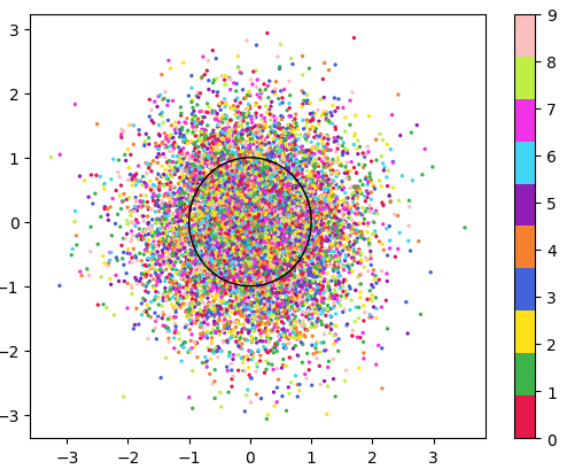
\includegraphics[width=.48\textwidth]{figures/1_component.PNG}
       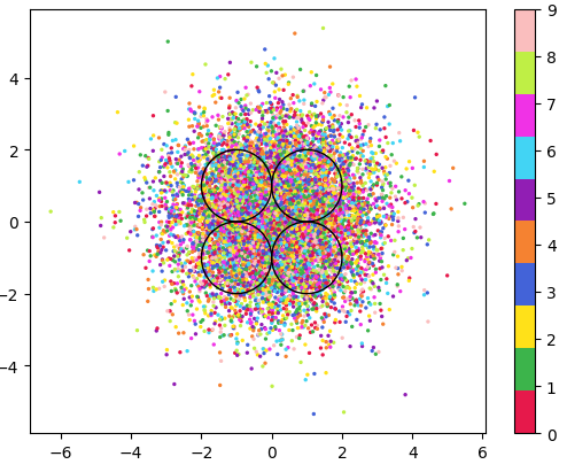
\includegraphics[width=.48\textwidth]{figures/4_components.PNG}
       \caption{Comparison of latent spaces for DML with unit prior (left) and DML with GMM prior containing 4 components (right) for $lsdim = 2$ on OrganAMNIST dataset. The gaussian components are shown as black with the raidus equal to variance (1). There appears to be no evidence of the distinct gaussian components in the latent space on the right. It does appear that the unit prior may regularize the magnitude of the latent vectors.}
       \label{fig:my_label}
   \end{figure}
   
    \section{Claim 3: Jointly Optimizing DML with VAE}
    To evaluate the third claim, we compare the performance of DMLs to MetricVAEs (defined in the previous chapter) across several metric losses. We run experiments for triplet loss, supervised loss, and center loss DML and MetricVAE models. To judge whether the claim is true, we will assess whether the model performance improves for the MetricVAE over the DML for the same metric loss and other hyper parameters. 
    
    \begin{table}
    \begin{tabular}{|c|c|c|c|c|c|c|c|c|c|}
            \hline
            & & & &  \multicolumn{2}{|c|}{\textbf{Triplet}} & \multicolumn{2}{|c|}{\textbf{Supervised}} & \multicolumn{2}{|c|}{\textbf{Center}}\\
            \hline
            \textbf{dataset} & \textbf{pl\%} & \textbf{lsdim} & \textbf{alpha} & \textbf{DML} & \textbf{MVAE} & \textbf{DML} & \textbf{MVAE} &
            \textbf{DML} &
            \textbf{MVAE}\\
            \hline
            MNIST & 0.01 & 2 & 0.25 & 0.2603 & 0.1025 & 0.3167 & 0.1052 & 0.1889 & 0.1001 \\
             & 0.01 & 2 & 0.50 & & 0.1049 & & 0.2699 & & 0.1034 \\
             & 0.01 & 2 & 0.75 & & 0.1004 & & 0.1055 & & 0.1064 \\
             & 0.01 & 2 & 1.00 & & 0.1115 & & 0.1022 & & 0.1004 \\
             & 0.01 & 10 & 0.25 & 0.2678 & 0.1028 & 0.5281 & 0.0947 & 0.5509  & 0.1064 \\
             & 0.01 & 10 & 0.50 & & 0.0923 & & 0.2630 & & 0.0995 \\
             & 0.01 & 10 & 0.75 & & 0.1037 & & 0.1040 & & 0.1076 \\
             & 0.01 & 10 & 1.00 & & 0.1067 & & 0.1040 & & 0.0932 \\
             & 10 & 2 & 0.25 & 0.4625 & 0.1109 & 0.1103 & 0.1028 & 0.1682 & 0.0992 \\
             & 10 & 2 & 0.50 & & 0.0992 & & 0.1073  & & 0.10467 \\
             & 10 & 2 & 0.75 & & 0.1031 & & 0.1022 & & 0.1001 \\
             & 10 & 2 & 1.00 & & 0.0890 & & 0.0920 & & 0.1010 \\
             & 10 & 10 & 0.25 & 0.8395 & 0.1025 & 0.9370 & 0.1010 & 0.46430 & 0.0986 \\
             & 10 & 10 & 0.50 & & 0.1025 & & 0.0932 & & 0.1073 \\
             & 10 & 10 & 0.75 & & 0.1058 & & 0.1043 & & 0.0947 \\
             & 10 & 10 & 1.00 & & 0.0950 & & 0.1076 & & 0.1013 \\
             
             OrganAMNIST & 0.01 & 2 & 0.25 & 0.3941 & 0.1061 & 0.3608 & 0.0911 & 0.1967 & 0.1061\\
             & 0.01 & 2 & 0.50 & & 0.0965 & & 0.1019 & & 0.1010  \\
             & 0.01 & 2 & 0.75 & & 0.0929 & & 0.1076 & & 0.1097\\
             & 0.01 & 2 & 1.00 & & 0.1010 & & 0.1055 & & 0.1040 \\
             
             & 0.01 & 10 & 0.25 & 0.6997 & 0.1175 & 0.4868 & 0.1058 & 0.5422 & 0.1121 \\
             & 0.01 & 10 & 0.50 & & 0.0929 & & 0.1094 & & 0.0989 \\
             & 0.01 & 10 & 0.75 & & 0.1091 & & 0.1112 & & 0.1040 \\
             & 0.01 & 10 & 1.00 & & 0.1091 & & 0.1007 & & 0.0911  \\
             
             & 10 & 2 & 0.25 & 0.4625 & 0.0968 & 0.6694 & 0.1091 & 0.2228 & 0.1061 \\
             & 10 & 2 & 0.50 & & 0.0995 & & 0.1067 & & 0.0965  \\
             & 10 & 2 & 0.75 & & 0.1061 & & 0.0959 & & 0.1613 \\
             & 10 & 2 & 1.00 & & 0.1043 & & 0.1679 & & 0.1007 \\
             
             & 10 & 10 & 0.25 & 0.8395 & 0.0980 & 0.9694 & 0.1091 & 0.5932 & 0.1094 \\
             & 10 & 10 & 0.50 & & 0.0980 & & 0.1238 & & 0.1019 \\
             & 10 & 10 & 0.75 & & 0.0974 & & 0.1346 & & 0.1148 \\
             & 10 & 10 & 1.00 & & 0.1025 & & 0.1076 & & 0.1088 \\
            \hline
       \end{tabular}
       \caption{Comparison of KNN Accuracy for DML and MetricVAE (MVAE) across metric losses for the MNIST dataset. The DML models do not take any alpha value, so their results are consistent across pl\% and lsdim. The pl\% value of 0.001 is not included as the supervised loss receives a NaN error. }
       \label{tab:my_label}
    \end{table}
    
    From table 6.5, we see that the MVAE for each loss only occasionally trains to perform better than the null model. The corresponding DML model almost always performs much better. This is true across all percentages of labelled data, latent space dimensionality, and alpha values. As with claim 2, it is possible this is because the training routine of alternating between supervised loss (in this case, metric loss) and unsupervised (in this case, VAE loss) is not optimal for training the model. Further supporting this point, previously we have received the following results for testing a version of the MVAE model that is trained against both the supervised and unsupervised loss on each epoch, as shown in table 6.6. In these results, we see clearly that an alpha value of over zero (i.e. incorporating both the supervised metric loss into the overall MVAE loss function) can help improve performance especially among lower dimensionalities. 
    
    \begin{figure}
        \centering
        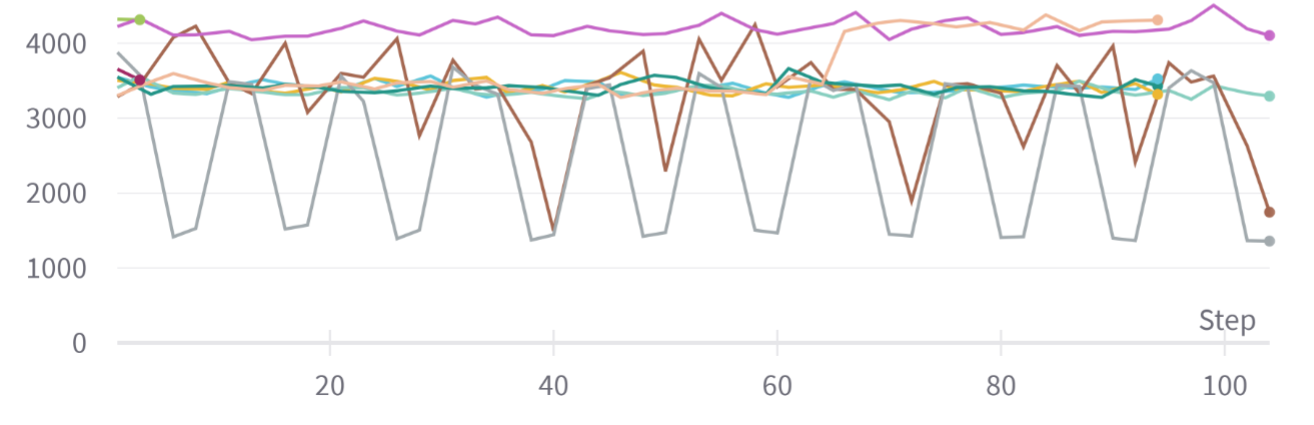
\includegraphics[width=.96\textwidth]{figures/recon_loss_convergence_cropped.png}
        \caption{Graph of reconstruction loss (componenet of unsupervised loss) of MVAE across epochs. The unsupervised loss does not converge despite being trained on each epoch.}
        \label{fig:my_label}
    \end{figure}
    
    Given our analysis of the data, we see that incorporating the DML loss to the VAE is potentially helpful, but only when training the unsupervised and supervised losses jointly. Even in that case, it is unclear whether the MVAE performs better than the corresponding DML model even if it does perform better than the corresponding VAE model. Alternating between training the model on the unsupervised and supervised objectives is does not appear to be a viable training routine. From the data and our analysis, we are unable to confirm the claim that optimizing a DML model jointly with a VAE on the VAE’s latent space will produce superior clustering than the DML model individually.
    
  \begin{table}
  \centering
    \label{tab:table1}
    \begin{tabular}{|c|c|c|c|c|c|c|c|}
      \hline
      \multicolumn{2}{|l|}{\textbf{\hspace{0.2cm} Architecture Parameters} \hspace{0.2cm}} & \multicolumn{3}{m|}{\textbf{MVAE Clasif. Accuracy (\%)}} & 
      \multicolumn{3}{m|}{\textbf{DML Clasif. Accuracy (\%)}}\\
      \hline
      \textbf{\hspace{0.4cm}  lsdim  \hspace{0.4cm}} & \textbf{gamma} & \textbf{linear} & \textbf{rf} & \textbf{kNN} & \textbf{linear} & \textbf{rf} & \textbf{kNN}\\
      \hline
       {} & 0 & 57.8 & 65.2 & 64.6 & & &\\ % <-- Combining 2 rows with arbitrary with (*) and content 12
      \multirow{2}
      & 2 & \textbf{75.0} & 69.8 & 70.6 & 95.0 & 94.5 & 95.0\\ % <-- Content of first column omitted.
      & 5 & 68.8 & 67.9 & 66.9 & & &\\
      & 10 & 51.6 & \textbf{75.4} & \textbf{74.2} & & &\\
      \hline
      {} & 0 & 81.3 & 83.9 & 84.5 & & &\\ % <-- Combining 2 rows with arbitrary with (*) and content 12
      \multirow{5}
      & 2 & 85.9 & 88.5 & 88.4 & 98.1 & 97.9 & 97.9\\ % <-- Content of first column omitted.
      & 5 & 82.8 & 88.0 & 88.5 & & &\\
      & 10 & \textbf{89.1} & \textbf{92.0} & \textbf{92.4} & & &\\
      \hline
      {} & 0 & 85.9 & 92.1 & 92.7 & & &\\ % <-- Combining 2 rows with arbitrary with (*) and content 12
      \multirow{10}
      & 2 & 87.4 & 91.8 & 91.3 & 98.5 & 97.7 & 98.0\\ % <-- Content of first column omitted.
      & 5 & \textbf{98.4} & \textbf{92.8} & \textbf{93.4} & & &\\
      & 10 & 93.8 & 92.5 & 91.9 & & &\\
      \hline
    \end{tabular}
    \caption{Experiments performed on MVAE architecture across fully labelled MNIST dataset that trains on objective function $L = L_{U} + \gamma * L_{S}$ on fully supervised dataset. The best results for the classification accuracy on the MVAE embeddings in a given latent-dimensionality are bolded.\\}
    \end{table}
    
    
    
\end{document}
